
% \section{联邦学习实践--Tensorflow federated}
 

% FATE架构如\ref{fate_architecture}所示. 
% \subsection{FATE架构及安装}
% \begin{figure}[htb]
%     \center
% 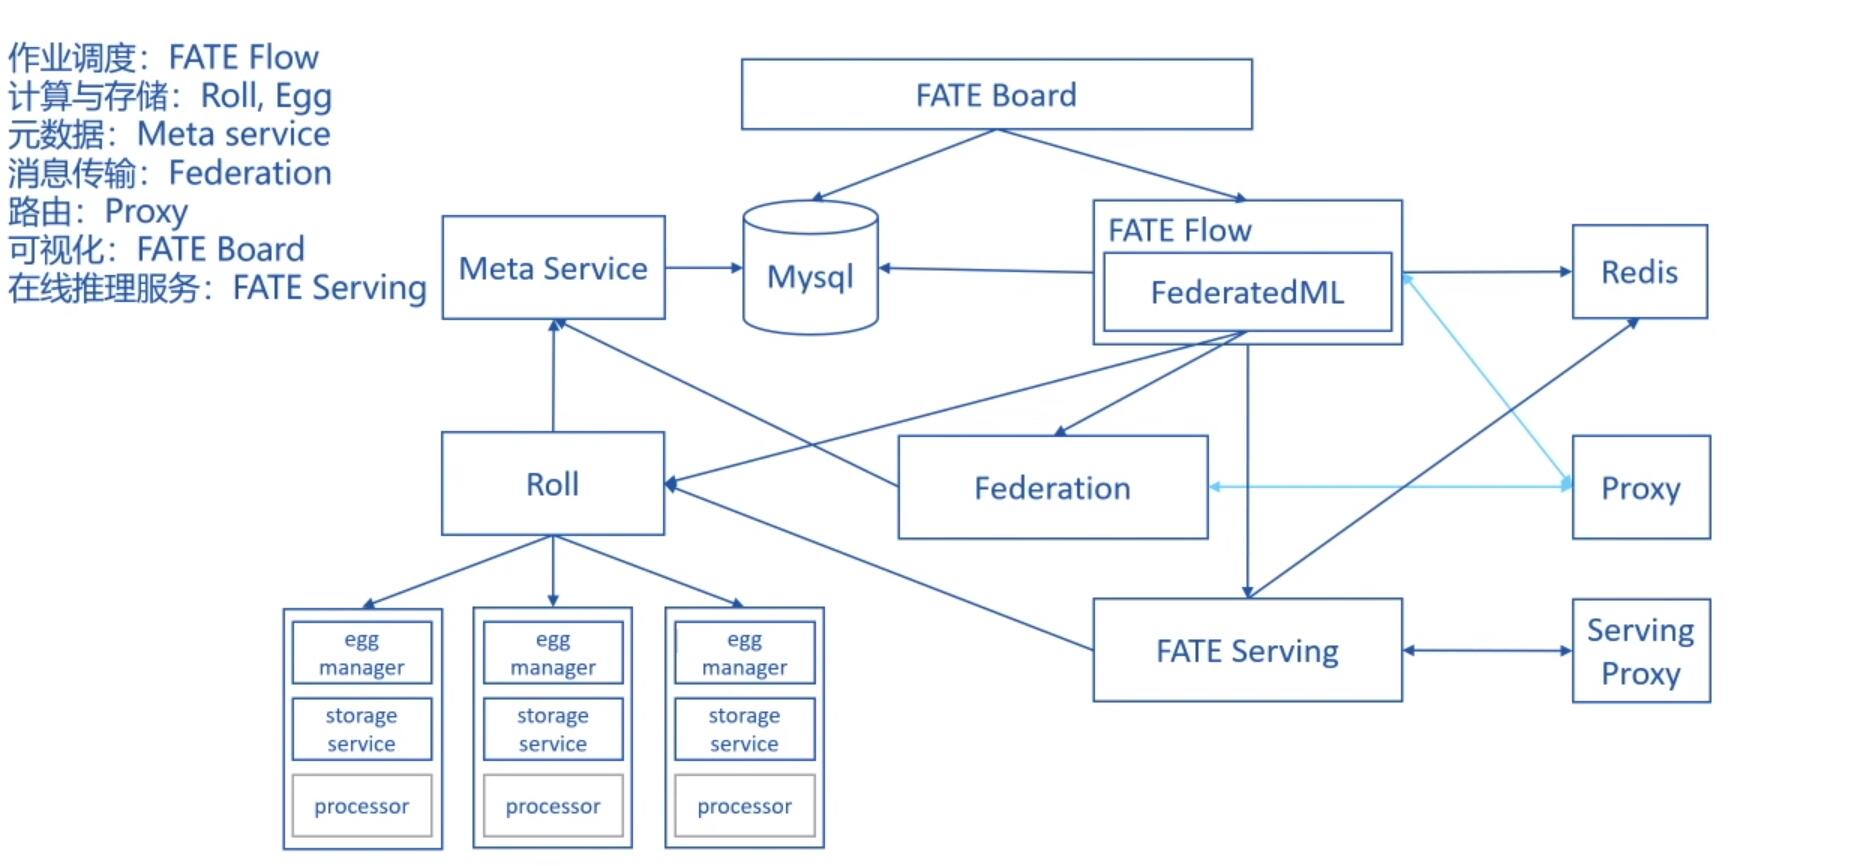
\includegraphics[width=0.8\textwidth]{fate1.jpg}
% \caption{联邦学习架构}
% \label{fate_architecture}
% \end{figure}

% \paragraph{准备工作}
% \begin{enumerate}
%     \item 两个主机(物理机或者虚拟机, 都是Ubuntu系统);
%     \item 所有主机安装Docker版本: 18+;
%     \item 所有主机安装Docker-Compose 版本: 1.24+;
%     \item 主机相互之间可以网络互通;
%     \item ssh免密登录
% \end{enumerate}
% 部署成功后使用 docker ps 命令显示如下组件, 分别对应于架构各部分. 
% \begin{figure}[!ht]
%     \center
% 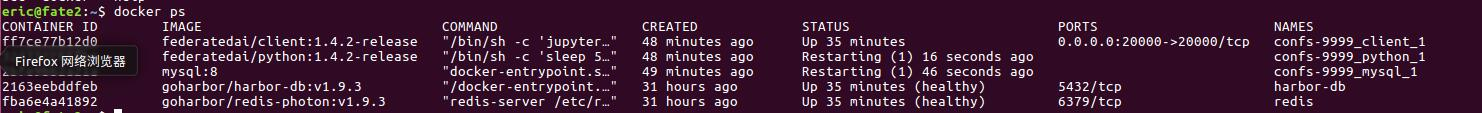
\includegraphics[width=0.8\textwidth]{fate_success.jpg}
% \caption{FATE运行时各组件}
% \end{figure}

% \subsection{实验-利用MINST数据集进行联邦学习训练-待做}

% \paragraph{初步计划}

% 将MINST数据集的6万调数据分为两个3万的数据集,在两台机器分别训练后再提交合并. 

\section{联邦学习实践-Tensorflow federated}


\textbf{联邦平均算法 -- 图像处理}

\paragraph{准备输入数据}

使用minst数据集的联邦学习版本

Leafproject  提供了对EMNIST和Shakespeare的预处理, 它还提供了sentiment140和celebA数据集的联邦版本. 这些数据集具有足够的客户端, 可以用于模拟跨设备FL场景, 但是对于规模特别重要的问题, 它们可能太小. 在这方面, Stackoverflow提供了跨设备FL问题的最现实示例.

 联邦学习需要联邦数据集,即来自多个用户的数据集合。 

为了便于进行实验,我们在TFF存储库中注入了一些数据集,其中包括MNIST的联邦版本,其中包含已使用Leaf重新处理过的原始NIST数据集的版本,以便数据的原始作者为数字。由于每个作者都有独特的风格,因此该数据集展现了联邦数据集所期望的非同伴行为(non-iid)。

数据是non-iid的, 用户通常拥有不同的数据分布。有些客户端在设备上的培训示例可能比较少,这会导致本地数据匮乏,而有些客户端会有足够多的培训示例。


\begin{figure}[!ht]
    \center
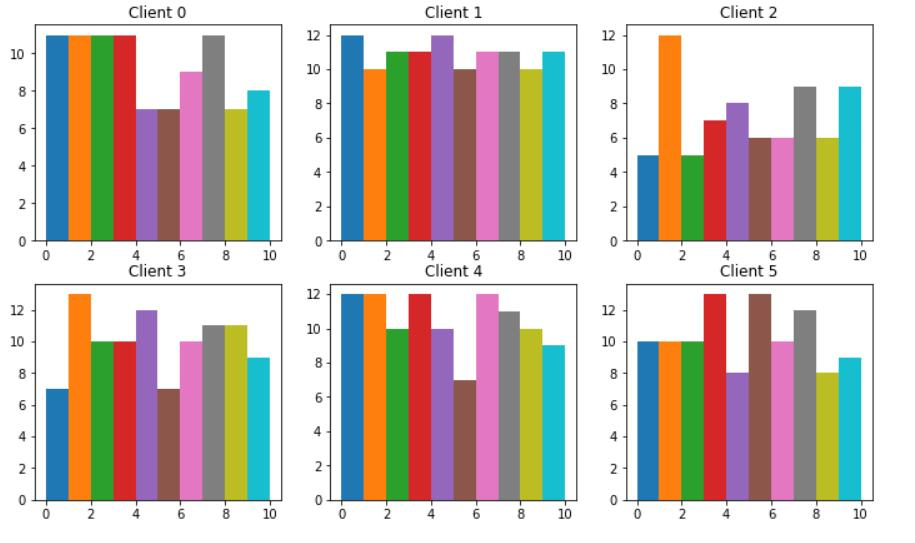
\includegraphics[width=0.4\textwidth]{figures/CDP/label_count.jpg}
\caption{客户端样本计数}
\label{fig:label_count}
\end{figure}
 由于每个人的独特书写风格,一个客户的数字平均图像(相当于本地聚合模型)与另一个客户的相同数字平均值图像看起来不同。
\ref{fig:mean_image}可视化了每个客户端每个MNIST标签的平均图像。
 
\begin{figure}[!ht]
    \center
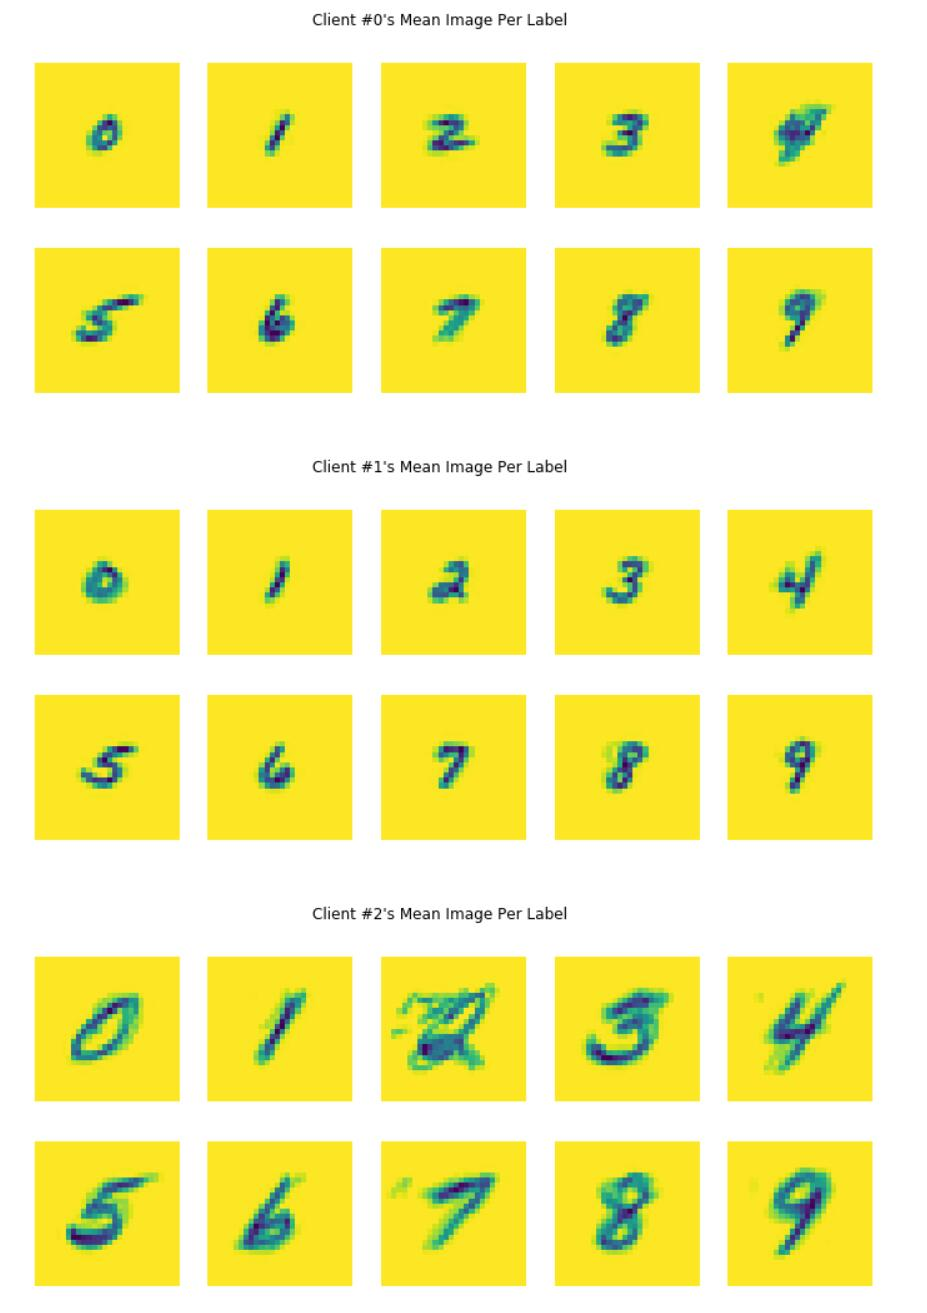
\includegraphics[width=0.4\textwidth]{figures/CDP/Mean_image.jpg}
\caption{客户端平均图像}
\label{fig:mean_image}
\end{figure}


\paragraph{选择客户-随机子抽样}
在典型的联邦培训场景中,我们正在处理大量潜在的用户设备,其中只有一小部分可以在给定的时间进行培训。例如,当客户端设备是仅在插入电源,已关闭计量网络且处于空闲状态时才参与培训的移动电话时,就是这种情况。

我们在模拟时,我们将简单地抽样要参与每一轮培训的客户的随机子集,通常每一轮都不同。 
相反,我们要做的是对一组客户端进行采样,并在各回合中重复使用同一组客户端,以加快收敛速度​​(有意将这些用户数据\textbf{过拟合})。 

\paragraph{创建模型}
使用Keras创建

\paragraph{训练模型}
使用client 和 server 优化器
client优化器仅用于计算每个客户端上的本地模型更新。server优化器将平均更新应用于服务器上的全局模型.
 
\begin{figure}[!ht]
    \center
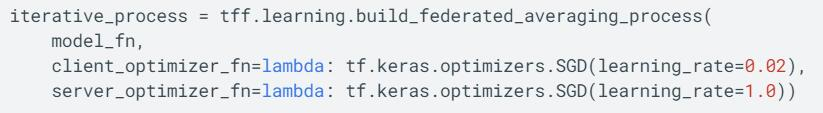
\includegraphics[width=0.4\textwidth]{figures/CDP/fedavgcode.jpg}
\label{fig:fedavgcode}
\end{figure}

\paragraph{结果}

在每轮联合训练之后,训练损失正在减少,表明该模型正在收敛

\paragraph{进一步实验}  

数据来自不同用户

自定义学习算法

% \subsection{并行模型}

% 数据并行(data parallelism):不同的机器有同一个模型的多个副本, 每个机器分配到不同的数据, 然后将所有机器的计算结果按照某种方式合并. 

% 数据并行化式的分布式训练在每个工作节点上都存储一个模型的备份, 在各台机器上处理数据集的不同部分. 数据并行化式训练方法需要组合各个工作节点的结果, 并且在节点之间同步模型参数. 

% 模型并行(model parallelism):分布式系统中的不同机器(GPU/CPU等)负责网络模型的不同部分 —— 例如, 神经网络模型的不同网络层被分配到不同的机器, 或者同一层内部的不同参数被分配到不同机器;
% \begin{figure}[!t]
%     \center
% 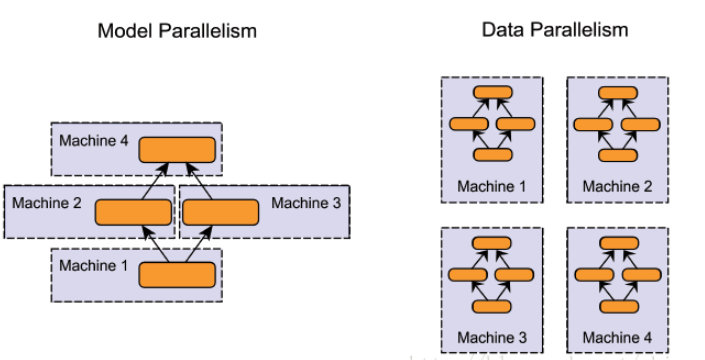
\includegraphics[width=0.6\textwidth]{paralle.png}
% \caption{并行模型}
% \label{parallelism}
% \end{figure}


% \subsubsection{AlexNet模型并行}
% AleaNe的训练需要由两个GPU卡井行完成. 在AexNet中, 卷积核被划分为两组, 分别在两块GPU上做模型并行训练. 不过, AlexNet对模型进行了一定的修改. 依照常规的模型并行逻辑, 每层神经网络的计算过程中都会发生通信, 然而在AlexNet中, 第一个卷积层到第二个卷积层、第三个卷积层到第四个卷积层以及第四个卷积层到第五个卷积层的两路计算之间没有依赖, 因而无须交互和通信. 这样做主要是为了减少通信的数据量, 提高并行的效率. 
% 基于模型井行的算法从直观上可以理解成把多个工作节点虚拟化为一个巨大的计算节点. 在计算过程中模型划分越多, 交互和通信也将越多, 并且任何一个工作节点出现问题整个计算都会受到影响, 因此鲁棒性欠佳. AlexNet 在提高效率方面进行了有益的尝试, 通过在模型设计中放弃些交互, 换来整体效率的提升. 

% 模型并行与联邦学习中模型的合并






